\section{Performance Evaluation}
\label{sec:performance-evaluation}

\definecolor{npc}{RGB}{150,150,150}
\definecolor{lvpc}{RGB}{66,133,244}
\definecolor{vac}{RGB}{244,160,0}
\definecolor{metac}{RGB}{52,168,83}
\definecolor{candc}{RGB}{171,71,188}
\pgfplotsset{
    perfbar/.style={
        ybar, ymin=0, ymajorgrids, grid style={gray!25},
        axis line style={gray!60}, tick style={gray!60},
        xtick=data, xtick pos=bottom, ytick pos=left,
        ticklabel style={font=\footnotesize},
        label style={font=\footnotesize},
        legend style={at={(0.5,1.02)}, anchor=south, legend columns=-1,
                      draw=none, font=\footnotesize,
                      /tikz/every even column/.append style={column sep=6pt}},
        nodes near coords,
        every node near coord/.append style={font=\tiny},
    },
}

\subsection{Experimental Methodology}
\label{subsec:performance-methodology}

\subsubsection{Simulation Configuration and Workloads}

All experiments use the baseline configuration of
Section~\ref{sec:impl-env} with the default memory timing
(\texttt{extraAssumedLat = 2}). The predictors are turned on through
configuration options.

I used twelve workloads: stable, random base, alternating value,
V-cache miss, stable flip, V-cache flip, none, forwarding cold, mixed,
store producer, forwarding both, and forwarding flip. The first four
share a chain of four dependent loads,
$P\rightarrow C\rightarrow E\rightarrow F$, where each load supplies
the next load's address. $P$ is the producer, $C$ is the dependent
consumer, and $E$ and $F$ are the third and fourth loads. On each lap,
conflict stores evict the chain lines from L1D. In the V-cache-miss
variant, the lines are 4~KiB apart, so they share a value-cache index.
These four workloads run 100 warm-up laps followed by 200 measured
laps. The counters agree with this: four chain loads per lap give 800
L1D read misses in the measured region.
Table~\ref{tab:workload-characteristics} describes all twelve
workloads.

\begin{table}[H]
    \centering
    \small
    \setlength{\tabcolsep}{4pt}
    \renewcommand{\arraystretch}{1.15}
    \caption{Workloads and what each one tests}
    \label{tab:workload-characteristics}
    \begin{tabularx}{\linewidth}{@{}>{\raggedright\arraybackslash}p{0.17\linewidth}>{\raggedright\arraybackslash}X>{\raggedright\arraybackslash}X@{}}
        \toprule
        \textbf{Workload} & \textbf{Pattern} & \textbf{What it tests} \\
        \midrule
        Stable & Addresses and values are the same every lap. &
        It is the best case for both LVP and V-ASTRA. \\
        Random base & $P$ reads a randomly chosen line, but all lines hold
        the same value. &
        LVP can predict the value, but $P$'s address is unpredictable. \\
        Alternating value & The value at $P$ changes every lap. &
        LVP cannot become confident, but V-ASTRA can still predict. \\
        V-cache miss & Chain lines map to the same value-cache entry. &
        V-ASTRA always misses, so only LVP can help. \\
        Stable flip & The value at $P$ changes every 32 laps. &
        It tests periodic LVP mispredictions and recovery. \\
        V-cache flip & It uses the V-cache-miss layout, and the value changes every
        32 laps. &
        It tests LVP recovery when V-ASTRA gives almost no benefit. \\
        None & Addresses and values are random. &
        It was meant to defeat both predictors. V-ASTRA still reduced
        cycles by 18.57\%. \\
        Forwarding cold & An older cold load stalls the pipeline before
        a dependent pair of loads. &
        It tests V-ASTRA bypass and forwarding to the dependent load. \\
        Mixed & A V-cache-miss chain is followed by a forwarding-cold
        segment. &
        LVP helps one part and V-ASTRA the other. META is faster than
        both. \\
        Store producer & An older store to a cold address precedes the stable chain. &
        It was meant to make META wait for V-ASTRA. This case did not
        occur. \\
        Forwarding both & It uses the forwarding layout with data already in the cache. &
        It tests forwarding when little latency is left to hide. The
        gain is small. \\
        Forwarding flip & It uses the forwarding layout, and the value changes every
        32 laps. &
        It tests forwarding with periodic LVP mispredictions. The gain
        is small. \\
        \bottomrule
    \end{tabularx}
\end{table}

\subsubsection{Measurement and Repetition}

The main metric is the number of cycles in the measured region. The
cycle reduction of a mode relative to no prediction (NP) is
\[
  \text{Reduction (\%)} =
  100*\,\frac{C_{\mathrm{NP}}-C_{\mathrm{mode}}}
  {C_{\mathrm{NP}}}.
\]

Each result was run five times with the same program, launched from
output paths of different lengths. The simulator is deterministic, so
almost all repeated runs gave exactly the same cycle count, and the
few differences were at most about 0.15\%. These repeats only check
how sensitive the results are to memory layout.

\subsection{Standalone Predictor Comparison}
\label{subsec:standalone-predictor-performance}

Figure~\ref{tab:standalone-predictor-cycles} compares LVP alone and
V-ASTRA alone on the first four workloads.

\begin{figure}[H]
    \centering
    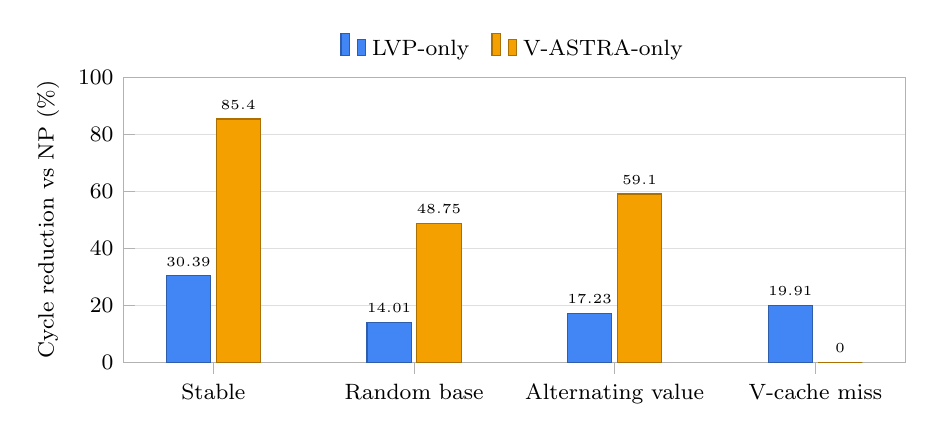
\begin{tikzpicture}
    \begin{axis}[perfbar, width=0.95\linewidth, height=5.2cm,
        bar width=16pt, ymax=100, enlarge x limits=0.15,
        ylabel={Cycle reduction vs NP (\%)},
        symbolic x coords={Stable,Random base,Alternating value,V-cache miss}]
        \addplot[fill=lvpc, draw=lvpc!70!black] coordinates
            {(Stable,30.39) (Random base,14.01) (Alternating value,17.23) (V-cache miss,19.91)};
        \addplot[fill=vac, draw=vac!70!black] coordinates
            {(Stable,85.40) (Random base,48.75) (Alternating value,59.10) (V-cache miss,0)};
        \legend{LVP-only, V-ASTRA-only}
    \end{axis}
    \end{tikzpicture}
    \caption{Cycle reduction of the standalone predictors relative to NP.
    NP takes 34,547, 35,608, 31,344, and 31,144 cycles on the four
    workloads, respectively.}
    \label{tab:standalone-predictor-cycles}
\end{figure}

V-ASTRA only helps when the value cache has the data. On stable,
all 800 chain loads were bypassed, and no L1D read misses were left. On random base, 595 loads
bypassed, and L1D read misses fell from 800 to 205. On V-cache miss,
all 800 lookups missed the value-cache tags, so there was no bypass
and no gain. No load used forwarding in these runs, so all of
V-ASTRA's gain here comes from the bypass itself. LVP gives smaller
but steady gains on all four workloads, including V-cache miss, where
V-ASTRA does not help at all.

Changing the measured region from 100 to 800 laps, with at least five
warm-up laps, changed the reductions by at most about 0.1 percentage
points.

\subsection{META Performance}
\label{subsec:meta-performance}

Figure~\ref{tab:meta-cycle-comparison} compares LVP alone, V-ASTRA
alone, and META on all twelve workloads, using the default
\texttt{off} mode for LVP-served loads.

\begin{figure}[H]
    \centering
    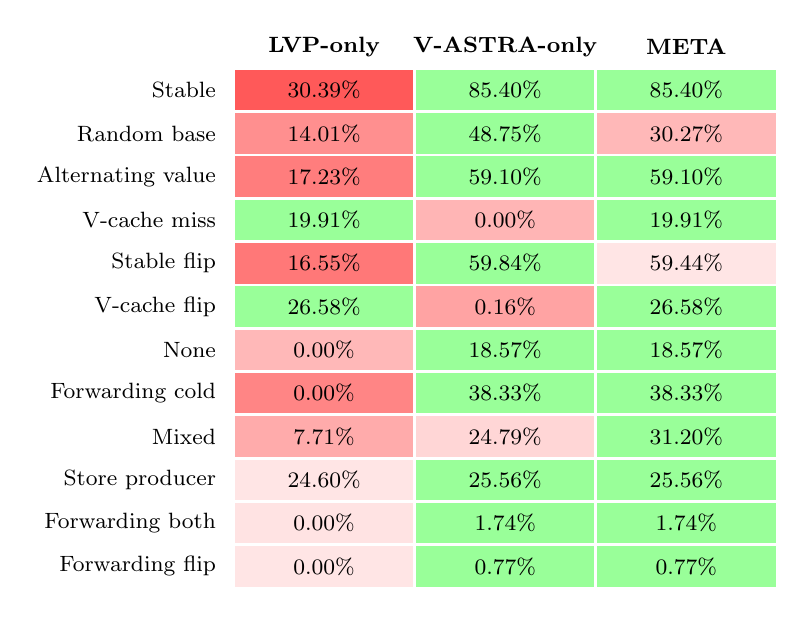
\begin{tikzpicture}[cell/.style={draw=white, line width=1pt,
        minimum width=2.30cm, minimum height=0.55cm, font=\footnotesize}]
    \node[font=\footnotesize\bfseries] at (4.15,0) {LVP-only};
    \node[font=\footnotesize\bfseries] at (6.45,0) {V-ASTRA-only};
    \node[font=\footnotesize\bfseries] at (8.75,0) {META};
    \node[anchor=east, font=\footnotesize] at (2.9,-0.55) {Stable};
    \node[cell, fill=red!65] at (4.15,-0.55) {30.39\%};
    \node[cell, fill=green!40] at (6.45,-0.55) {85.40\%};
    \node[cell, fill=green!40] at (8.75,-0.55) {85.40\%};
    \node[anchor=east, font=\footnotesize] at (2.9,-1.10) {Random base};
    \node[cell, fill=red!44] at (4.15,-1.10) {14.01\%};
    \node[cell, fill=green!40] at (6.45,-1.10) {48.75\%};
    \node[cell, fill=red!28] at (8.75,-1.10) {30.27\%};
    \node[anchor=east, font=\footnotesize] at (2.9,-1.65) {Alternating value};
    \node[cell, fill=red!51] at (4.15,-1.65) {17.23\%};
    \node[cell, fill=green!40] at (6.45,-1.65) {59.10\%};
    \node[cell, fill=green!40] at (8.75,-1.65) {59.10\%};
    \node[anchor=east, font=\footnotesize] at (2.9,-2.20) {V-cache miss};
    \node[cell, fill=green!40] at (4.15,-2.20) {19.91\%};
    \node[cell, fill=red!29] at (6.45,-2.20) {0.00\%};
    \node[cell, fill=green!40] at (8.75,-2.20) {19.91\%};
    \node[anchor=east, font=\footnotesize] at (2.9,-2.75) {Stable flip};
    \node[cell, fill=red!53] at (4.15,-2.75) {16.55\%};
    \node[cell, fill=green!40] at (6.45,-2.75) {59.84\%};
    \node[cell, fill=red!10] at (8.75,-2.75) {59.44\%};
    \node[anchor=east, font=\footnotesize] at (2.9,-3.30) {V-cache flip};
    \node[cell, fill=green!40] at (4.15,-3.30) {26.58\%};
    \node[cell, fill=red!36] at (6.45,-3.30) {0.16\%};
    \node[cell, fill=green!40] at (8.75,-3.30) {26.58\%};
    \node[anchor=east, font=\footnotesize] at (2.9,-3.85) {None};
    \node[cell, fill=red!28] at (4.15,-3.85) {0.00\%};
    \node[cell, fill=green!40] at (6.45,-3.85) {18.57\%};
    \node[cell, fill=green!40] at (8.75,-3.85) {18.57\%};
    \node[anchor=east, font=\footnotesize] at (2.9,-4.40) {Forwarding cold};
    \node[cell, fill=red!48] at (4.15,-4.40) {0.00\%};
    \node[cell, fill=green!40] at (6.45,-4.40) {38.33\%};
    \node[cell, fill=green!40] at (8.75,-4.40) {38.33\%};
    \node[anchor=east, font=\footnotesize] at (2.9,-4.95) {Mixed};
    \node[cell, fill=red!33] at (4.15,-4.95) {7.71\%};
    \node[cell, fill=red!16] at (6.45,-4.95) {24.79\%};
    \node[cell, fill=green!40] at (8.75,-4.95) {31.20\%};
    \node[anchor=east, font=\footnotesize] at (2.9,-5.50) {Store producer};
    \node[cell, fill=red!10] at (4.15,-5.50) {24.60\%};
    \node[cell, fill=green!40] at (6.45,-5.50) {25.56\%};
    \node[cell, fill=green!40] at (8.75,-5.50) {25.56\%};
    \node[anchor=east, font=\footnotesize] at (2.9,-6.05) {Forwarding both};
    \node[cell, fill=red!11] at (4.15,-6.05) {0.00\%};
    \node[cell, fill=green!40] at (6.45,-6.05) {1.74\%};
    \node[cell, fill=green!40] at (8.75,-6.05) {1.74\%};
    \node[anchor=east, font=\footnotesize] at (2.9,-6.60) {Forwarding flip};
    \node[cell, fill=red!10] at (4.15,-6.60) {0.00\%};
    \node[cell, fill=green!40] at (6.45,-6.60) {0.77\%};
    \node[cell, fill=green!40] at (8.75,-6.60) {0.77\%};
    \end{tikzpicture}
    \caption{Cycle reduction relative to NP for LVP-only, V-ASTRA-only,
    and META (\texttt{metaAstraLvpLoads=off}). Green marks the largest
    reduction for each workload. Red shading grows with the gap, in
    percentage points, to that largest reduction.}
    \label{tab:meta-cycle-comparison}
\end{figure}

META matches the better of the two predictors on nine of the twelve
workloads, and on mixed it beats both, with a 31.20\% reduction. Mixed
is where combining helps most, because LVP serves one part of the lap
and V-ASTRA the other. On random base and stable flip, however, META
is slower than V-ASTRA alone: 24,828 versus 18,249 cycles on random
base, and 13,039 versus 12,912 on stable flip. So combining the
predictors does not always give the best result. These measurements
alone do not explain every difference, but the random-base case is
examined in the next subsection.

\subsection{Provisional-Base Modes on the Random-Base Workload}
\label{subsec:provisional-base-performance}

To find out why META loses on random base, I ran it in all three
modes of Section~\ref{sec:impl-provisional}.
Figure~\ref{tab:randbase-mode-cycles} shows the cycle reductions and
L1D read misses.

\begin{figure}[H]
    \centering
    \pgfplotsset{rbmode/.style={perfbar, width=0.52\linewidth, height=5.4cm,
        bar width=13pt, enlarge x limits=0.13,
        symbolic x coords={NP,V-ASTRA,off,train,candidate},
        xticklabels={No pred.,V-ASTRA,META off,META train,META cand.},
        xticklabel style={rotate=35, anchor=north east, font=\footnotesize}}}
    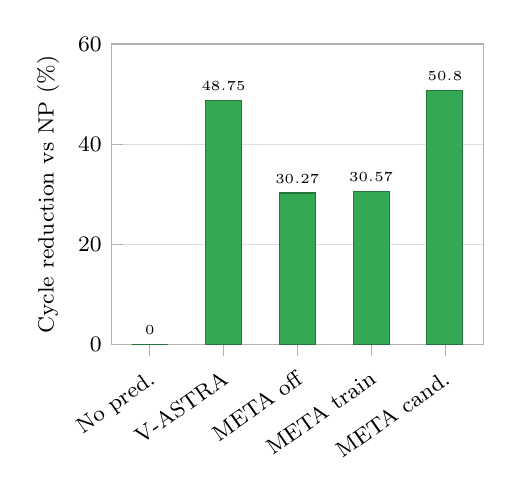
\begin{tikzpicture}
    \begin{axis}[rbmode, ymax=60, ylabel={Cycle reduction vs NP (\%)},
        nodes near coords={\pgfmathprintnumber[fixed,precision=2]{\pgfplotspointmeta}}]
        \addplot[fill=metac, draw=metac!70!black] coordinates
            {(NP,0) (V-ASTRA,48.75) (off,30.27) (train,30.57) (candidate,50.80)};
    \end{axis}
    \end{tikzpicture}\hfill
    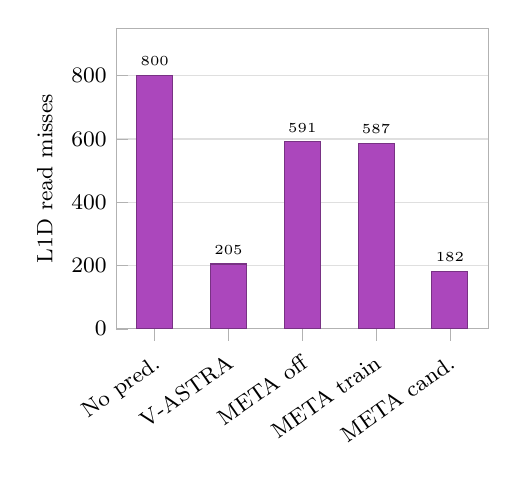
\begin{tikzpicture}
    \begin{axis}[rbmode, ymax=950, ylabel={L1D read misses}]
        \addplot[fill=candc, draw=candc!70!black] coordinates
            {(NP,800) (V-ASTRA,205) (off,591) (train,587) (candidate,182)};
    \end{axis}
    \end{tikzpicture}
    \caption{Random-base cycle reduction relative to NP (left) and L1D
    read misses (right) across provisional-base modes.}
    \label{tab:randbase-mode-cycles}
\end{figure}

Figure~\ref{tab:randbase-mode-events} shows the matching event
counts. In this workload, every V-ASTRA candidate also bypassed, so
the candidate count equals the number of bypasses.

\begin{figure}[H]
    \centering
    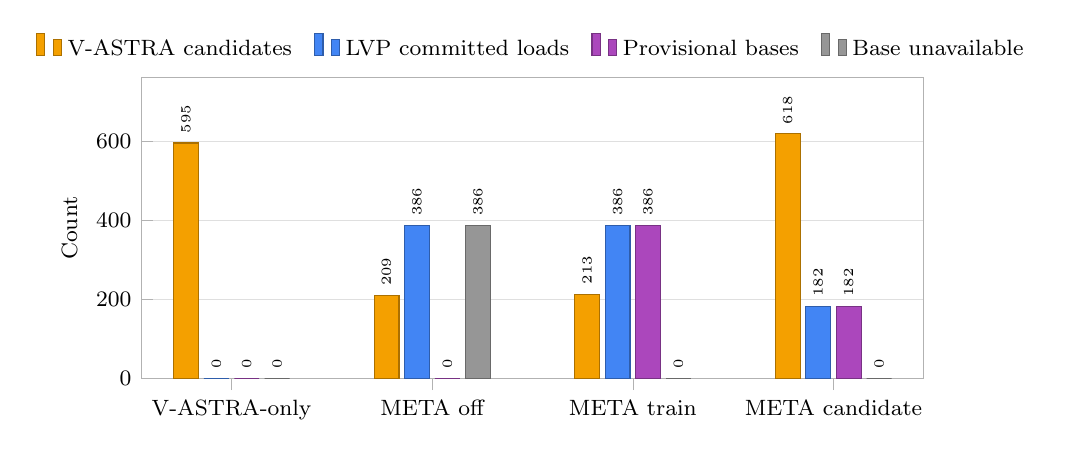
\begin{tikzpicture}
    \begin{axis}[perfbar, width=0.95\linewidth, height=5.4cm,
        bar width=9pt, ymax=760, enlarge x limits=0.15,
        every node near coord/.append style={font=\tiny, rotate=90, anchor=west},
        ylabel={Count},
        symbolic x coords={V-ASTRA-only,META off,META train,META candidate}]
        \addplot[fill=vac, draw=vac!70!black] coordinates
            {(V-ASTRA-only,595) (META off,209) (META train,213) (META candidate,618)};
        \addplot[fill=lvpc, draw=lvpc!70!black] coordinates
            {(V-ASTRA-only,0) (META off,386) (META train,386) (META candidate,182)};
        \addplot[fill=candc, draw=candc!70!black] coordinates
            {(V-ASTRA-only,0) (META off,0) (META train,386) (META candidate,182)};
        \addplot[fill=npc, draw=npc!70!black] coordinates
            {(V-ASTRA-only,0) (META off,386) (META train,0) (META candidate,0)};
        \legend{V-ASTRA candidates, LVP committed loads,
                Provisional bases, Base unavailable}
    \end{axis}
    \end{tikzpicture}
    \caption{Random-base event counts. Every provisional base was
    validated and none was dropped. V-ASTRA-only has no LVP.}
    \label{tab:randbase-mode-events}
\end{figure}

In \texttt{off} mode, LVP serves 386 loads, and none of them can
become V-ASTRA candidates. This leaves only 209 candidates, compared
with 595 for V-ASTRA alone. The \texttt{train} mode changes little,
with only 106 fewer cycles than \texttt{off}. The \texttt{candidate}
mode is much faster. It needs 7,310 fewer cycles than \texttt{off}
(29.4\%) and 731 fewer than V-ASTRA alone. It raises the number of
bypasses from 209 to 618, cuts L1D read misses from 591 to 182, and
reduces the loads served by LVP from 386 to 182.

\subsection{Performance of Dependency-Handling Designs}
\label{subsec:dependency-performance}

These experiments use the default timing (\texttt{extraAssumedLat =
2}), so Design~A has no effect here and is not measured. Design~B is
turned on together with V-ASTRA, and there was no V-ASTRA run without
forwarding to compare against. Figure~\ref{tab:forwarding-performance} shows V-ASTRA with
forwarding against NP on the four forwarding workloads. The number
under each workload counts loads admitted to forwarding, not
committed instructions.

\begin{figure}[H]
    \centering
    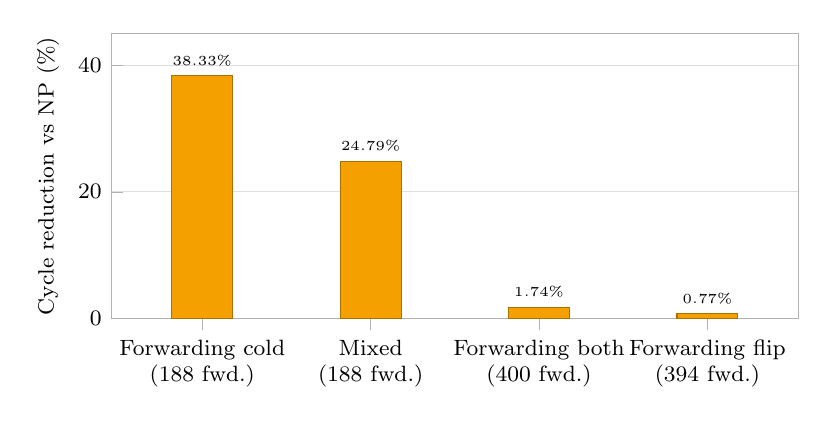
\begin{tikzpicture}
    \begin{axis}[perfbar, width=0.85\linewidth, height=5.2cm,
        bar width=22pt, ymax=45, enlarge x limits=0.18,
        ylabel={Cycle reduction vs NP (\%)},
        symbolic x coords={fc,mx,fb,ff},
        xticklabels={{Forwarding cold\\(188 fwd.)},{Mixed\\(188 fwd.)},
                     {Forwarding both\\(400 fwd.)},{Forwarding flip\\(394 fwd.)}},
        xticklabel style={align=center},
        nodes near coords={\pgfmathprintnumber[fixed,precision=2]{\pgfplotspointmeta}\%}]
        \addplot[fill=vac, draw=vac!70!black] coordinates
            {(fc,38.33) (mx,24.79) (fb,1.74) (ff,0.77)};
    \end{axis}
    \end{tikzpicture}
    \caption{Cycle reduction of V-ASTRA with forwarding relative to NP on
    the forwarding workloads. The number under each workload is the
    number of loads admitted to forwarding.}
    \label{tab:forwarding-performance}
\end{figure}

On forwarding cold, cycles drop by 38.33\%, yet L1D read misses stay
at 400, even with 191 bypasses. The gain seems to come from
overlapping the cold misses rather than from avoiding them, although
the measurements cannot isolate this. On forwarding both and
forwarding flip, the gains are small (1.74\% and 0.77\%), with a
run-to-run variation of about 0.06\% and 0.15\% on those workloads.

\subsection{Threats to Validity and Interpretation}
\label{subsec:performance-limitations}

These results come from small deterministic microbenchmarks on one
MinorCPU, cache, and memory configuration, so they are not
application-level speedups. The repeated runs only test sensitivity to
memory layout, and are not independent statistical samples. Design~A
was not measured under the default timing, and Design~B's share of
the gain cannot be separated from V-ASTRA.

Overall, the cycle reductions are large but depend strongly on the
workload. META beats both predictors on mixed, but is slower than
V-ASTRA alone on random base and stable flip. Candidate mode gives a
large improvement on random base.
